\newpage
\section{Launch Phase}
\subsection{General Analysis}
	\subsubsection{Requirements	 Analysis}
	Run through these steps several times:\\
	Capture Requirements - Analyse Requirements - Specify Requirements - Verify Requirements.
		\begin{figure}[h!]		%Remember to put the h!, to not fuck the sections.
			\begin{centering}
				 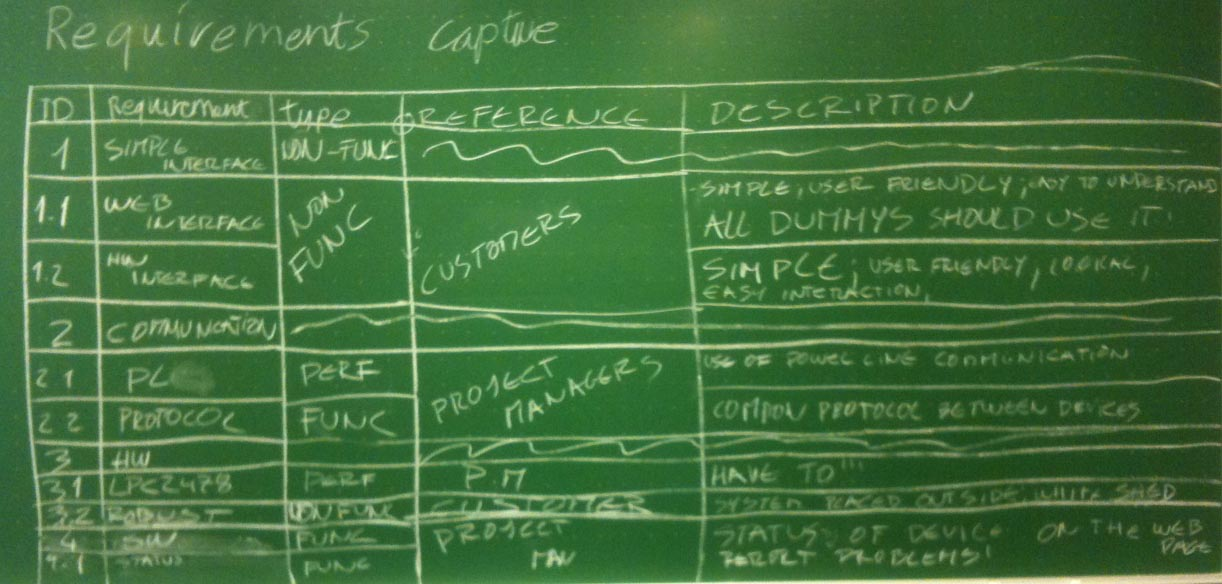
\includegraphics[width=1.0\textwidth]{images/requirement_capture.JPG}
		 		\caption{Design}
			 \end{centering}
		\end{figure}
		\begin{itemize}
			\item Functional Requirements ("system shall do 'requirement' ")
				\begin{itemize}
					\item
				\end{itemize}
			\item Non-functional Requirements ("system shall be 'requirement' ")
				\begin{itemize}
					\item something					
				\end{itemize}
			\item Behavioural Requirements ("how the system shall react")
				\begin{itemize}
					\item something
				\end{itemize}
			\item Performance Requirements ("how well does it have to be done")
				\begin{itemize}
					\item Easy to use and fast to learn web-user interface. Should be able to be used by non-technical persons.
				\end{itemize}
		\end{itemize}
		Put in diagrams of requirement capture (looks like class diagrams with inherited classes).\\
		Alternatively put in the requirements as in the picture we made on the blackboard.
	\subsubsection{Problem Domain Analysis}
			Make diagrams describing the parts that the hub should control, this is done by some kind of classes.
		\begin{itemize}
			\item Block Diagram\\
			\item State Machine Diagrams
		\end{itemize}
	\subsubsection{Usage Domain Analysis}
		\begin{itemize}
			\item Use Cases
		\end{itemize}
	\subsubsection{Interface Analysis}
		\begin{itemize}
			\item User Interface Descriptions
			\item System Interface Descriptions
		\end{itemize}
	\subsubsection{Function Analysis}
		\begin{itemize}
			\item Recognise the direction of the device ( input, output, both ).
			\item Start / Stop slave devices from web interface or physical module ( Control over the connected modules ).
			\item Routes energy from the input to output ports.
			\item Control power status of slave modules.
			\item Log device data ( uptime of the port and power amount since connected ).
			\item More to add here...
		\end{itemize}
	\subsubsection{System Dynamics}
		\begin{itemize}
			\item Communication Diagram
			\item Sequence Diagram
		\end{itemize}
	\subsubsection{General Analysis Specification}
\subsection{General Architecture Design}
	\subsubsection{Design Criteria}
	\subsubsection{Subsystem Design}
		\begin{itemize}
			\item Subsystem Architecture Diagram
			\item Detailed Block Diagrams
		\end{itemize}
	\subsubsection{Architecture Dynamics}
		\begin{itemize}
			\item Sequence Diagrams
		\end{itemize}
	\subsubsection{Architectural Specification and Constraints}
\subsection{Technical Platform}
	\subsubsection{Hardware Specifications}
	\subsubsection{Software Specifications}